\chapter{Background}


\section{Compiler Infrastructure}

Compilers are programming tools responsible for translating programs in a given source language to a lower-level target language.
This compilation process must preserve the program semantics.
Moreover, compilers are also expected to produce a good quality representation of the program in the target language, optimising for a given objective function.
An important objective function is code size, i.e., the optimisation goal is to produce a representation of the program as small as possible.

Compilers are usually organised in \textit{three-phases}, as shown in Figure~\ref{fig:3-phase-compiler}: frontend, optimiser, and backend.
The frontend is responsible for parsing, validating and diagnosing errors in the source code.
This parsed source code is then translated into an intermediate representation, which is the LLVM IR in this case.
The optimiser is responsible for doing a broad variety of transformations, that are usually independent of language and target machine, to improve the code's performance.
The backend, also known as the code generator, then translates the code from the intermediate representation onto the target instruction set.
It is common for the backend to also perform some low-level optimisations that take advantage of unusual features of the supported architecture.
%Common parts of a compiler backend include instruction selection, register allocation, and instruction scheduling.

\begin{figure}[h]
  \centering
  \includegraphics[scale=0.9]{src/background/figs/3-phase-compiler.pdf}
  \caption{Overview of the three-phase compiler infrastructure.}
  \label{fig:3-phase-compiler}
\end{figure}

However, these \textit{three-phases} represent only a simplified view of their designed.
In order to manage the complexity involved in optimising compilers, modern compilers are usually designed in a highly modular manner, where they are organised as a series of phases that sequentially analyse and transform the program being compiled.
For example, the frontend is subdivided into multiple phases.
The \textit{lexer} is responsible for tokenising the input stream of characters from the source code.
This token stream is then consumed by the \textit{parser}, producing a language-specific \textit{Abstract Syntax Tree} (AST).
The AST is an intermediate representation used during the semantic analysis, before being lowered to another intermediate representation.

\begin{figure}[h]
  \centering
  \includegraphics[scale=0.9]{src/background/figs/compiler-frontend.pdf}
  \caption{Breakdown of the frontend, illustrating how compilers are organised as a series of phases.}
  \label{fig:compiler-frontend}
\end{figure}

\begin{figure}[h]
\centering
\begin{subfigure}{\textwidth}
\centering
  \includegraphics[scale=0.9]{src/background/figs/ir-lowering-sequence.pdf}
  \caption{Sequence of representations used by modern compilers.}
  \label{fig:ir-lowering-sequence-general}
\end{subfigure}
\begin{subfigure}{\textwidth}
\centering
  \includegraphics[scale=0.9]{src/background/figs/ir-lowering-sequence-example.pdf}
  \caption{Overview of the three-phase compiler infrastructure.}
  \label{fig:ir-lowering-sequence-example}
\end{subfigure}
\caption{Example of identical functions.}
\label{fig:ir-lowering-sequence}
\end{figure}

Several intermediate representations, with different levels of abstraction, are used during this compilation process from the source to the target language.
Different analyses and optimisations are better modelled at different abstraction levels.
Figure~\ref{fig:ir-lowering-sequence-general} illustrates the sequence of representations used by modern compilers, each one having a progressively lower level than the previous one.
The source language is parsed into an AST, which is then commonly lowered to a high-level intermediate representation (HIR).
As shown in Figure~{fig:ir-lowering-sequence-example}, this HIR is usually a language-specific IR, such as the Swift Intermediate Language (SIL), which is used to solve domain-specific problems~\cite{lattner20}.
A popular mid-level intermediate representation (MIR) is the LLVM IR, which is shared among many compilers.
In the LLVM compiler infrastructure, the LLVM IR is lowered into a low-level representation (LIR), called the Machine IR, which is then lowered into the target assembly language.
This final process might actually involve multiple intermediate representations depending on the backend being used.


\subsection{Link-Time Optimisations}
%% benefits of LTO
%% challenges with LTO
%% mention partial LTO, such as ThinLTO

Figure~\ref{fig:full-pipeline} illustrates the standard pipeline for the compilation of multiple source files.
Compilers normally operate on a single translation unit at a time, where a translation unit includes a single source file and its expanded headers.
Each translation unit is optimised separately and compiled into a single native object file.
Finally, the linker combines multiple object files into a resulting binary or library.

\begin{figure}[h]
  \centering
  \includegraphics[scale=0.85]{src/background/figs/full-pipeline.pdf}
  \caption{Overview of the three-phase compiler infrastructure.}
  \label{fig:full-pipeline}
\end{figure}

However, this approach limits the impact of inter-procedural optimisations (IPO) to within each individual translation unit.
For example, if we have two identical functions defined in different translation units, they will not be merged using the approach shown in Figure~\ref{fig:full-pipeline}.
In order to achieve larger benefits from IPO, the optimisation scope can be increased to include multiple translation units.
When the scope includes all translation units being linked into an executable, the compiler can perform  more aggressive optimisations that rely on whole-program information~\cite{johnson17}.

\begin{figure}[h]
  \centering
  \includegraphics[scale=0.85]{src/background/figs/full-pipeline-LTO.pdf}
  \caption{Overview of the three-phase compiler infrastructure.}
  \label{fig:full-LTO-pipeline}
\end{figure}

Figure~\ref{fig:full-LTO-pipeline} illustrates a common mechanism for enabling whole-program optimisation called link-time optimisation (LTO).
In this approach, optimisations are applied in two different moments.
First, we have \textit{early} optimisations being applied on a per translation unit basis.
However, we also have \textit{late} optimisations being applied after all translation units are linked together.
Therefore, allowing important inter-procedural optimisations to be applied on the whole-program, across translation units.

In the LTO mode, compilers delay the generation of native object files.
As shown in Figure~\ref{fig:full-LTO-pipeline}, all translation units are linked while still in an IR better suited for the late optimisations.


%\section{Optimisation Scope}
%% describe local optimisations (block level), global (intra-procedural), and inter-procedural (across functions)

%\subsection{Interprocedural Optimisations}
%% benefits of IPO
%% challenges involved in IPO



\section{Sequence Alignment}

The comparison of two or more sequences, measuring the extent to which they differ, is important in many scientific areas, most notably in molecular biology~\cite{needleman70,smith81,carrillo88,wang94} where it has been critical
in the understanding of functional, structural, or evolutionary relationships between the sequences~\cite{kruskal83,mount05book}.

A particularly important comparison technique is sequence alignment, which identifies a series of patterns that appear in the same order in the sequences.
Essentially, sequence alignment algorithms insert blank characters in both input sequences so that the final sequences end up having the same size, where equivalent segments are aligned with their matching segments from the other sequence and non-equivalent segments are either paired with the blank or a mismatching character.

Figure~\ref{fig:seq-align-example} shows an example of a pair-wise sequence alignment.
This example, adapted from Lee~et~al.~\cite{lee02}, shows two protein sequences where amino acids are represented by their one-letter symbology~\cite{aasland68}.

\begin{figure}[h]
  \centering
  \includegraphics[scale=0.55]{src/background/figs/seq-align-example}
  \caption{Example of an optimum alignment between two sequences.
  Matching segments are shown in green, vertically centred, and the non-matching segments are shown in red at the sides.}
  \label{fig:seq-align-example}
\end{figure}

Formally, sequence alignment can be defined as follows:
For a given alphabet $\alpha$, a sequence $S$ of $k$ characters is an element of
$\alpha^k$, i.e., $S = (a_1, \ldots a_k)$.
Let $S_1, \ldots, S_m$ be a set of sequences, possibly of different lengths but
all derived from the same alphabet $\alpha$, where
$S_i = (a_1^{(i)}, \ldots, a_{k_i}^{(i)})$, for all $i\in\{1,\ldots,m\}$.
Consider an extended alphabet that includes the \textit{blank} character ``$-$'',
i.e., $\beta = \alpha \cup \{-\}$.
An alignment of the $m$ sequences, $S_1, \ldots, S_m$, is another set of sequences,
$\bar{S}_1, \ldots, \bar{S}_m$, such that each sequence $\bar{S}_i$ is obtained
from $S_i$ by inserting blanks in positions where some of the other sequences
have non-blank and possibly equivalent characters, for a given equivalence relation.
All sequences $\bar{S}_i$ in the alignment set have the same length $l$, where
$\max\{k_1,\ldots,k_m\} \leq l \leq k_1 + \cdots + k_m$.
Moreover, $\forall i\in\{1,\ldots, m\}$, $\bar{S}_i = (b_1^{(i)},\ldots,b_l^{(i)})$,
there are increasing functions $v_i: \{1,\ldots,k_i\} \to \{1,\ldots,l\}$, such that:
\begin{itemize}
\item $b_{v_i(j)}^{(i)} = a_j^{(i)}$, for every $j \in \{1,\ldots,k_i\}$;
\item any position not covered by the function $v_i$ contain a black character, i.e., for every $j \in \{1,\ldots,l\}\setminus \textrm{Im} \, v_i$, $b_j$ is the blank character ``$-$''.
\end{itemize}
Finally, for all $j\in\{1,\ldots,l\}$, there is at least one value of $i$ for which $b_j^{(i)}$ is not a blank character.
Note that two aligned sequences may contain both non-blank and non-equivalent characters at any given position, in which case there is a mismatch.

The sequence alignment problem is concerned with identifying an alignment that maximises the score for a given scoring scheme.
The scoring scheme first defines a weight for the alignment of pairs of characters which will then be used to compose a score for the whole sequence alignment.
These weights are used to penalise mismatches and gaps while favouring matching pairs.

The alignment score between two characters is defined by a function on pairs of characters, $\delta \in \beta\times\beta \to \mathbb{R}$, for a given extended alphabet $\beta$.
The simplest function that is commonly used is the constant function~\cite{haque09}.
Let $a,b\in\beta$ and $a \neq b$.
This constant function is defined by a triple $(w_1,w_2,w_3)\in\mathbb{R}^+\times\mathbb{R}^-\times\mathbb{R}^-$, such that:
\begin{itemize}
\item For two matching caracters, $\delta(a,a) = w_1, w_1\in\mathbb{R}^+$.
\item For a mismatch betweem non-blank characters, $\delta(a,b) = w_2, w_2\in\mathbb{R}^-$.
\item The gap penalty, for when we have a blank character, $\delta(a,-) = \delta(-,a) = w_3, w_3\in\mathbb{R}^-$.
\end{itemize}
This is a simple scoring scheme that rewards matches and penalises mismatches and gaps.

There is a vast literature on algorithms for performing sequence alignment, especially in the context of molecular biology.
These algorithms are classified as either global or local.
A global sequence alignment algorithm attempts to align the entire sequence, using as many characters as possible, up to both ends of each sequence.
Global alignment algorithms are useful for sequences that are highly similar and have approximately the same length~\cite{mount05book}.
Alternatively, a local sequence alignment algorithm generates subalignments in stretches of sequence with the highest density of matches.
Local alignments are more suitable for aligning sequences with very few similarities or vastly different lengths~\cite{mount05book}.

In this work, we will focus on pair-wise global alignment algorithms.
The following sections describe the main optimal algorithms based on dynamic programming.
These algorithms will offer different optimality, performance, and memory usage trade-offs~\cite{needleman70,smith81,carrillo88,hickey11}.
%Different alignments would produce different but valid merged functions.

\subsection{Needleman-Wunsch Algorithm}

The Needleman-Wunsch algorithm~\cite{needleman70} is one of the most well known algorithm for pair-wise global alignment.
This algorithm gives an alignment that is guaranteed to be optimal for a given scoring scheme~\cite{higgins89}.

The Needleman-Wunsch algorithm is based on dynamic programming and consists of two main steps.
First, it builds a \textit{similarity matrix}, based on a scoring scheme, which assigns weights for matches, mismatches, and \textit{gaps} (blank characters).
Afterwards, a backward traversal is performed on the similarity matrix, in order to reconstruct the final alignment by maximizing the total score.

\begin{figure}[h]
  \centering
  \includegraphics[scale=0.6]{src/background/figs/seq-align-example-nw}
  \caption{Example of the \textit{similarity matrix} computed for two input sequences.
           The highlighted cells represent the resulting alignment computed by the Needleman-Wunsch algorithm.}
  \label{fig:seq-align-example-nw}
\end{figure}

Figure~\ref{fig:seq-align-example-nw} shows the similarity matrix corresponding to the example from Figure~\ref{fig:seq-align-example}.
The similarity matrix is constructed by comparing all possible pairs of characters from the input sequences.
Let $S_1$ and $S_2$ be our input sequences of sizes $k_1$ and $k_2$, respectively, where $S_1 = (a_1,\ldots,a_{k_1})$ and $S_2 = (b_1,\ldots,b_{k_2})$.
The similarity matrix $M$ computed for these two input sequences will have size $(k_1 + 1) \times (k_2+1)$.
Let $M_{i,j}$ denote all entries in the similarity matrix, with $1 \leq i \leq (k_1 + 1)$ and $1 \leq j \leq (k_2 + 1)$.
The first entry in the matrix is $M_{1,1} = 0$, and
\begin{equation*}
%\begin{align*}
M_{i,j} = \max \begin{cases}
  M_{i-1,j} + \delta(a_{i-1},-)         &  \quad  \text{if } i>1 \text{ and } j\geq1 \\
  M_{i,j-1} + \delta(-,b_{j-1})         &  \quad  \text{if } i\geq1 \text{ and } j>1 \\
  M_{i-1,j-1} + \delta(a_{i-1},b_{j-1}) &  \quad  \text{if } i>1 \text{ and } j>1
\end{cases}
%\end{align*}
\end{equation*}
In other words, the score for each cell in the similarity matrix is the maximum among the rules shown in Figure~\ref{fig:seq-align-rules}.

\begin{figure}[h]
  \centering
  \includegraphics[scale=0.8]{src/background/figs/seq-align-rules}
  \caption{Set of rules used to compute the scores of the similarity matrix.
           The two first rules represent the penalty of inserting a horizontal or vertical gap.
           The diagonal rule depends whether we have a matching or mismatching pair of input characters.}
  \label{fig:seq-align-rules}
\end{figure}


Figure~\ref{fig:seq-align-example-nw} also highlights the traversal. 
Note that sometimes, while traversing the score matrix, there are multiple adjacent neighbours with the same score.
Since there may exist multiple traversals with the same score, two sequences can have multiple optimum alignments.

Needleman-Wunsh algorithm is quadratic in the size of the sequences being aligned, both in time and space.

%\subsection{Hirschberg Algorithm}


\section{Machine Learning}

Machine learning (ML) is the field of study of mathematical models that can automatically learn patterns from sample data, known as \textit{training} data, in order to make predictions for unseen data.
It is commonly seen as a subset of artificial intelligence and a superset of deep-learning (DL), which is a family of machine learning methods based on artificial neural networks.

Artificial neural networks (ANNs) are machine learning models that were vaguely inspired by the biological neural networks.
These models are composed of artificial neurons, which are essentially mathematical functions known as \textit{activation functions}, mapping inputs to a single output that can be fed to multiple other neurons.
These neurons are then connected by weighted edges.
Figure~\ref{fig:ML-feed-forward-network} shows a simple ANN with multiple layers of neurons, with fully connect layers, i.e., a neuron has an edge to every neuron in the next layer.

\begin{figure}[h]
  \centering
  \includegraphics[scale=0.85]{src/background/figs/ML-feed-forward-network.pdf}
  \caption{Example of an artificial neural network with multiple layers of neurons. Each circle represents an artificial neuron. Adjacent layers of neurons are fully connected.}
  \label{fig:ML-feed-forward-network}
\end{figure}

Machine learning is used in Chapter~\ref{chp:deeplearning} to classify input sequences.
This section describes the classification and sequential modelling techniques used in this thesis

Classification concerns the mapping of input variables to a categorical label.
The training of a classifier requires inputs for which the category is known, called labelled training data.

%Sequence modelling concerns the process of capturing the underlying probability distribution that describes the input sequences.


\subsection{Feed-forward Neural Networks}

\subsection{Recurrent Neural Networks}

\subsubsection{Gated Recurrent Units}
